\problemname{Bar Shelf}

\illustration{.4}{img/cropped_bottles.png}{A perfectly civilised arrangment of bottles. 
Detail from \emph{Dictionnaire encyclopédique de l'épicerie et des industries annexes} by Albert Seigneurie, 1904, p.~117. Public domain.}

Organ pipes, the von Trapp children, staircases---oh, how your boss loves these things.
For they are neatly arranged ascending order, the very signal of cleanliness, structure, \emph{civilisation}.
Were it up to him, the bottles on the bar shelf would all be neatly and propery ordered, left-to-right, and in ascending order.

The patrons at the bar, of course, disagree.
They much prefer a certain amount of messiness in how the bottles are organised, which communicates a welcoming atmosphere of carefully orchestrated insouciance. 

This has led to long discussions between you and your boss about how messy the shelf can be.
After all, a bottle placed to the left of one that is just slightly smaller doesn't look very messy at all.
On the other hand, even you have to admit that very big size differences do look pretty messy.
Finally, you have agreed on the following rule:
A pair of bottles, not necessarily adjacent, is a \emph{messy pair} if the left one is more than twice as large as the right one.

\medskip
For instance, in the image below, the bottles have height $4$, $5$, $2$, $1$, and $3$, from left to right.
The bottles of height $4$ and $1$ form a messy pair (because $4 > 2\cdot 1$), but $4$ and $2$ do not (because $4\not> 2\cdot 2$).
The height-$5$ bottle forms two messy pairs, with $1$ and $2$, respectively.
The bottles of height $1$ and $3$ are not messy, since the smaller one is nicely placed the right of the larger one, just as your boss likes it.

\medskip
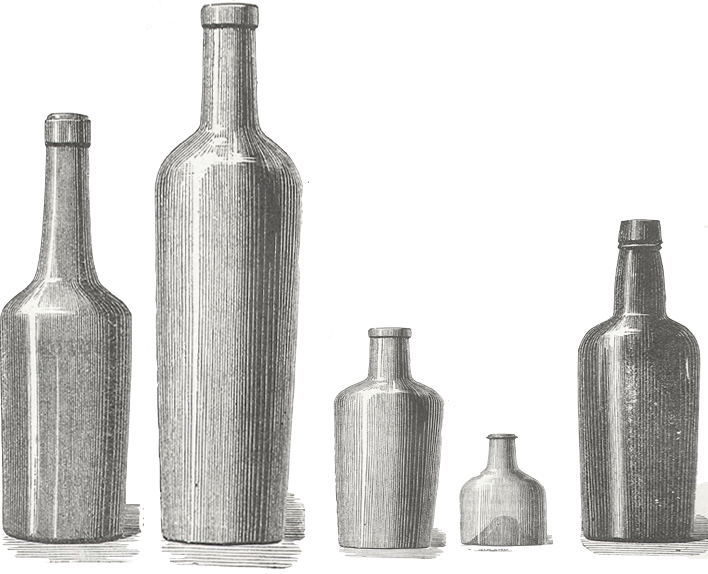
\includegraphics[width = 5cm]{img/messy_bottles.png}

The messiness of the entire shelf is the number of messy pairs.
In the above example, there were three messy pairs.


\section*{Input}

The input consists of two lines.
On the first line, the number $n$ of bottles on the shelf, where $n\in\{1,\ldots, 10^5\}$.
On the second line, $n$ integers, separated by space, giving the height (in nanometers) of the $n$ bottles from left to right.
Each height is an integer between $1$ and $10^9$.

\section*{Output}

Output a single integer: the messiness of the shelf.
